\documentclass[aspectratio=169]{beamer}%[handout]
\usepackage[T1]{fontenc}
\usepackage[utf8]{inputenc}
\usepackage[spanish,es-tabla]{babel}
\usepackage{beamerthemeshadow,beamerthemesplit,cite,cancel,lmodern,eso-pic,fancyvrb,textcomp,times,booktabs,amssymb,amsmath,ragged2e,float,subfig,xspace,epic,eepic,multicol,multirow,colortbl,color,graphicx,url,hyperref,array,appendixnumberbeamer,listings,pgfpages}
\usepackage[normalem]{ulem} %tachar texto con \sout{}

\setcounter{tocdepth}{3}
\usepackage[figurename=]{caption}


%%%%%%%%%%%%%%%%%%%%%%%%%%%
%TEXTDRAW COMPILAR CON XELATEX
%%%%%%%%%%%%%%%%%%%%%%%%%%%
\usepackage[usenames,dvipsnames]{pstricks}
\usepackage{pstricks-add}
\usepackage{epsfig}
\usepackage{pst-grad} % For gradients
\usepackage{pst-plot} % For axes
\usepackage[space]{grffile} % For spaces in paths
\usepackage{etoolbox} % For spaces in paths
\makeatletter % For spaces in paths
\patchcmd\Gread@eps{\@inputcheck#1 }{\@inputcheck"#1"\relax}{}{}
\makeatother


\mode<handout>{
\pgfpagesuselayout{4 on 1}[letterpaper,border shrink=5mm, landscape]
}

%Colores Ulagos
%COLOREAR SISTEMA
\definecolor{gray97}{gray}{.97}
\definecolor{gray75}{gray}{.75}
\definecolor{gray45}{gray}{.45}
\definecolor{listinggray}{gray}{0.9}
\definecolor{lbcolor}{rgb}{0.9,0.9,0.9}
\definecolor{amarillo}{RGB}{255,182,18}
\definecolor{verde}{RGB}{52,178,51}
\definecolor{rojo}{RGB}{237,41,57}
\definecolor{azulu}{RGB}{19,83,139}
\definecolor{azul}{RGB}{0,91,187}
\definecolor{negro}{RGB}{35,31,32}
\definecolor{naranjo}{RGB}{251,79,20}
\definecolor{morado}{RGB}{143,35,179}
\definecolor{gris}{RGB}{183,177,169}
%COLOREAR TEXTO
\newcommand\rojo[1]{\textcolor[RGB]{237,41,57}{#1}}
\newcommand\gris[1]{\textcolor[RGB]{183,177,169}{#1}}
\newcommand\azul[1]{\textcolor[RGB]{0,91,187}{#1}}
\newcommand\verde[1]{\textcolor[RGB]{52,178,51}{#1}}
\newcommand\naranjo[1]{\textcolor[RGB]{251,79,20}{#1}}
\newcommand\amarillo[1]{\textcolor[RGB]{255,182,18}{#1}}
\newcommand\morado[1]{\textcolor[RGB]{143,35,179}{#1}}
\newcommand\negro[1]{\textcolor[RGB]{35,31,32}{#1}}


\newcommand\cita[1]{{\scriptsize \begin{flushright}\emph{(#1)}\end{flushright}}}%formato cita: \cita{texto}

\newcommand{\ignore}[1]{} %comentario multilinea

%%%%%%%%%%%%%%%%%%%%%%%%%
%% Tikz
%%%%%%%%%%%%%%%%%%%%%%%%%
\usepackage{tikz}
\usetikzlibrary{trees}
\usetikzlibrary{decorations.pathmorphing}
\usetikzlibrary{arrows}
\usetikzlibrary{shapes}
\usetikzlibrary{backgrounds}
\usetikzlibrary{patterns}
\usetikzlibrary{fit}
\usetikzlibrary{positioning} % LATEX and plain TEX
%%%%%%%%%%%%%%%%%%%%%%%%%%

%%%%%%%%%%%%%%%%%%%%%TEMA
\mode<presentation>
\usetheme{CambridgeUS}
\usecolortheme[named=azul]{structure}
\useinnertheme{rectangles}
\useoutertheme{infolines}
\setbeamercovered{transparent}
\setbeamerfont{block title}{size={}}
\setbeamerfont{title}{shape=\scshape}
\setbeamerfont{frametitle}{shape=\scshape}
\setbeamerfont{author}{shape=\scshape}
\setbeamerfont{institute}{shape=\scshape}
\setbeamerfont{block title}{shape=\scshape}
\setbeamertemplate{blocks}[rounded][shadow=true]
\setbeamertemplate{itemize items}[default]
\setbeamertemplate{enumerate items}[circle]
\setbeamertemplate{description item}[align left]
\setbeamertemplate{blocks}[rounded][shadow=true]
\setbeamertemplate{title page}[default][colsep=-4bp,rounded=false,shadow=false]
\setbeamercolor*{palette primary}{use=structure,fg=azulu,bg=gray97}%texto titulo y fecha
\setbeamercolor*{palette secondary}{use=structure,fg=azulu,bg=gray97}%fondo titulo abajo
\setbeamercolor*{palette tertiary}{use=structure,fg=gray97,bg=azulu}
\setbeamercolor*{title}{use=structure,fg=white}%Portada
\setbeamercolor*{author}{use=structure,fg=white}%Portada
\setbeamercolor*{institute}{use=structure,fg=white}%Portada
\setbeamercolor*{date}{use=structure,fg=white}%Portada
\setbeamercolor{frametitle right}{bg=azul!50!white}
\setbeamercolor{structure}{fg=azul}
%Bloques
\setbeamercolor{block title}{use=structure,fg=white,bg=amarillo}
\setbeamercolor{block body}{use=structure,fg=negro,bg=amarillo!20!white}
\setbeamercolor{block title example}{use=structure,fg=white,bg=verde!80!black}
\setbeamercolor{block body example}{use=structure,fg=negro,bg=verde!20!white}
\setbeamercolor{block title alerted}{use=structure,fg=white,bg=rojo!90!negro}
\setbeamercolor{block body alerted}{use=structure,fg=negro,bg=rojo!20!white}
\newtheorem{sintaxis}{Sintaxis}
\AtBeginEnvironment{sintaxis}{%
  \setbeamercolor{block title}{use=structure,fg=white,bg=morado}
  \setbeamercolor{block body}{use=structure,fg=negro,bg=morado!20!white}
}
\newtheorem{resultado}{Resultado}
\AtBeginEnvironment{resultado}{%
  \setbeamercolor{block title}{use=structure,fg=negro,bg=gris}
  \setbeamercolor{block body}{use=structure,fg=negro,bg=gris!20!white}
}
\setbeamertemplate{background}{\centering
\includegraphics[height=9cm,width=16cm]{fondoula}}
%%%%%%%%%%%%%%%%%%%%%FIN TEMA

%lstlisting %%%%%CODIGOS
\lstset{tabsize=2,language=SQL,basicstyle=\small,keywordstyle=\color{azul}, commentstyle= \scriptsize\color{verde},showstringspaces=false, stringstyle=\color{red},breaklines=true,literate={á}{{\'a}}1 {é}{{\'e}}1 {í}{{\'i}}1 {ó}{{\'o}}1 {ú}{{\'u}}1
  {Á}{{\'A}}1 {É}{{\'E}}1 {Í}{{\'I}}1 {Ó}{{\'O}}1 {Ú}{{\'U}}1
  {à}{{\`a}}1 {è}{{\`e}}1 {ì}{{\`i}}1 {ò}{{\`o}}1 {ù}{{\`u}}1
  {À}{{\`A}}1 {È}{{\'E}}1 {Ì}{{\`I}}1 {Ò}{{\`O}}1 {Ù}{{\`U}}1
  {ä}{{\"a}}1 {ë}{{\"e}}1 {ï}{{\"i}}1 {ö}{{\"o}}1 {ü}{{\"u}}1
  {Ä}{{\"A}}1 {Ë}{{\"E}}1 {Ï}{{\"I}}1 {Ö}{{\"O}}1 {Ü}{{\"U}}1
  {â}{{\^a}}1 {ê}{{\^e}}1 {î}{{\^i}}1 {ô}{{\^o}}1 {û}{{\^u}}1
  {Â}{{\^A}}1 {Ê}{{\^E}}1 {Î}{{\^I}}1 {Ô}{{\^O}}1 {Û}{{\^U}}1
  {œ}{{\oe}}1 {Œ}{{\OE}}1 {æ}{{\ae}}1 {Æ}{{\AE}}1 {ß}{{\ss}}1
  {ű}{{\H{u}}}1 {Ű}{{\H{U}}}1 {ő}{{\H{o}}}1 {Ő}{{\H{O}}}1
  {ç}{{\c c}}1 {Ç}{{\c C}}1 {ø}{{\o}}1 {å}{{\r a}}1 {Å}{{\r A}}1
  {€}{{\EUR}}1 {£}{{\pounds}}1 {Ñ}{{\~N}}1 {ñ}{{\~n}}1 {¿}{{?`}}1}

%%%%%%%%%%%%%%PORTADA
\title[Métodología de Desarrollo]{\textbf{\huge{Métodología de Desarrollo}}}
\subtitle{Modelamiento y Paradigmas de Programación}
\author[Juan José Ramírez Lama]{\small{\textbf{Juan José Ramírez Lama}\\ \texttt{juan.ramirez@ulagos.cl}}}
\institute[ULagos]{\small{\textbf{Departamento de Ciencias de la Ingeniería}\\Ingeniería Civil en Informática}}
\date[\today]{}
%%%%%%%%%%%%%FIN PORTADA

\graphicspath{images/}

\begin{document}
%Pagina de Portada
\begin {frame} [plain]
\maketitle
\end {frame}


\setbeamertemplate{background}{}
%%%%%%%%%%%%%%%%ÍNDICES
\section[Contenido]{}
\frame{
  \frametitle{\textbf{Tabla de Contenido}}
\setcounter{tocdepth}{2}%1: solo titulo principal, 2: titulo y subtitulo, 3....
\tableofcontents[]}
%Generacion de Indice por capitulo
\AtBeginSection[]{
\begin{frame}
\frametitle{\textbf{Sección Siguiente}}
\tableofcontents[currentsection]
\end{frame}}
%presentar subseccion
%\AtBeginSubsection[]{
%\begin{frame}
%\frametitle{\textbf{Contenido}}
%\tableofcontents[currentsection,currentsubsection]
%\end{frame}}
%%%%%%%%%%%%%%%%FIN ÍNDICES

\begin{frame}[fragile]
\frametitle{\textbf{Etapas de Propuesta del Proyecto}}
\justifying

\begin{enumerate}
 \item Concebir idea de proyecto.
 \item Plantear el problema a resolver con el proyecto.
  \begin{itemize}
   \item Establecer los Objetivos.
   \item Desarrollar las preguntas de investigación.
   \item Justificar el desarrollo y su viabilidad.
   \item Establecer la Metodología de trabajo.
  \end{itemize}
\item Elaborar el Marco Teórico.
\begin{itemize}
 \item Revisión de la literatura.
 \begin{itemize}
 \item Detección
 \item Obtención
 \item Consulta
 \item Extracción y recopilación de la información de interés.
 \end{itemize}
 \item Construcción del marco teórico.
 \begin{itemize}
  \item Comparativa
  \item Puntos de mejora.
 \end{itemize}

\end{itemize}

\end{enumerate}
\end{frame}

\section{Ídea de Proyecto}


\begin{frame}[fragile]
\frametitle{\textbf{Concebir Idea de Proyecto}}
\justifying
Cualquier proceso para idear un proyecto implica:
\begin{itemize}
 \item Observar
 \item Describir
 \item Explicar
 \item Predecir
\end{itemize}
\end{frame}

\begin{frame}[fragile]
\frametitle{\textbf{Observación}}
\justifying
\begin{itemize}
 \item El \rojo{objeto de nuestro proyecto} es cualquier objeto, situación acontecimiento o cosa, sobre la cual fijaremos nuestra atención.
 \item Comprender las características, interrelaciones o establecer conexiones, entre el problema y otros modos para conocer su comportamiento en el contexto que lo rodea.
 \item Verificar lo que se quiere desarrollar (conocer la competencia del mercado).
\end{itemize}
\end{frame}

\begin{frame}[fragile]
\frametitle{\textbf{Describir}}
\justifying
\begin{itemize}
 \item Permite \rojo{reunir los resultados de la observación}
 \item Agrupa y convierte en información, hechos y eventos que caracterizan la realidad observada
 \begin{itemize}
  \item Los hechos empíricos se convierten en datos susceptibles de medir y comparar
 \end{itemize}
\end{itemize}
\end{frame}

\begin{frame}[fragile]
\frametitle{\textbf{Explicar}}
\justifying
\begin{itemize}
 \item Establecer relaciones entre rasgos de un objeto, situación, acontecimiento, entre otros.
 \item Para esto es necesario utilizar la información dada por la descripción y las observaciones que se han realizado.
\end{itemize}
\end{frame}

\begin{frame}[fragile]
\frametitle{\textbf{Predecir}}
\justifying
\begin{itemize}
 \item Es la consecuencia de la explicación.
 \item Predecir es poder anticipar sobre la base de las explicaciones logradas acerca del comportamiento de los fenómenos, la ocurrencia y modo de manifestarse si se dan condiciones previamente conocidas.
\end{itemize}
\end{frame}

\begin{frame}[fragile]
\frametitle{\textbf{Interrogantes para iniciar el proceso}}
\justifying

\begin{center}
\begin{tabular}{|p{7cm}|p{7cm}|}
\hline
\textbf{Preguntas}&\textbf{Área Asociada del Informe}\\\hline
¿Qué Desarrollar?& Definición del tema/Introducción \\\hline
¿Cuál es la situación actual?&Planteamiento del problema \\\hline
¿Qué cosas deben ser solucionadas?&Formulación del proyecto \\\hline
¿Qué propósitos el proyecto?& Objetivos \\\hline
¿Qué motiva el desarrollo?&Justificación y aporte \\\hline
¿Quienes han realizado herramientas similares?¿Qué las caracterizan?& Marco Teórico \\\hline
¿Cómo se va a realizar el proyecto?&Metodología de trabajo\\\hline
¿Cuánto tiempo se va a emplear en el desarrollo del proyecto?& Carta Gantt y Actividades\\\hline
¿Qué fuentes se van a referir?&Bibliografía\\\hline
\end{tabular}
\end{center}
\end{frame}

\begin{frame}[fragile]
\frametitle{\textbf{Idear un proyecto}}
\justifying
\begin{itemize}
 \item Las ideas de un proyecto pueden surgir luego de:
\begin{itemize}
 \item Observación (ciudadanía, prácticas, vivencias, entre otros)
 \item Después de leer un artículo, noticia, entre otros.
 \item Al estudiar un tema.
 \item Conversar con otras personas.
 \item etc.
\end{itemize}
\item Toda instancia es válida para plantearse una idea de proyecto.
\end{itemize}
\end{frame}

\begin{frame}[fragile]
\frametitle{\textbf{Buenas Ideas de proyecto}}
\justifying
\begin{itemize}
 \item Proyectos que motivan de manera personal y/o profesional.
 \item Ideas que no necesariamente son nuevas, pero si novedosas, por añadir mejoras, perspectivas no tratadas o reinvensión de un proyecto.
 \item En la investigación, sirven para elaborar teorías y posibles soluciones a problemas, o generar nuevas interrogantes y cuestionamientos.
 \item \textbf{Son solicitadas por una empresa o entidad que respalda el proceso}.
\end{itemize}

\end{frame}


\section{Planteamiento del Problema}


\subsection{Objetivos}
\begin{frame}[fragile]
\frametitle{\textbf{Objetivos}}
\justifying
\begin{itemize}\justifying
 \item Se deben abordar desde el principio del proyecto, expresan los fines que se esperan lograr con el estudio del problema planteado, responden a la pregunta \naranjo{¿Para qué se lleva a cabo el proyecto?}, por lo general comienzan con un verbo en infinitivo: Determinar, identificar, establecer, distinguir, medir, cuantificar, entre otros.

\item Deben enunciar un resultado unívoco, preciso, factible y medible. Su formulación debe ser clara, concisa y bien orientada hacia el fin, en función de ellos se plantean los métodos de recolección de datos, pruebas estadísticas, entre otros.

\item Evitar unir objetivos, idealmente, un objetivo general y varios específicos.
\end{itemize}

\end{frame}

\begin{frame}[fragile]
\frametitle{\textbf{Preguntas/ideas}}
\justifying
\begin{itemize}
 \item El planteamiento de las preguntas se realiza directamente a partir de los objetivos específicos planteados.
\item Cada objetivo específico se ``mapea'' a una idea/pregunta del proyecto.
\end{itemize}


\begin{exampleblock}{Por ejemplo:}
  \begin{itemize}
  \item \textbf{\naranjo{Objetivo:}} Optimizar los métodos de acceso a disco.
  \item \textbf{\naranjo{Pregunta:}} ¿Cuáles son los métodos de acceso a disco?
\end{itemize}
\end{exampleblock}

\begin{exampleblock}{Por ejemplo:}
  \begin{itemize}
  \item \textbf{\naranjo{Objetivo:}} Descubrir las competencias que poseen los líderes efectivos de algunas empresas Chilenas.
  \item \textbf{\naranjo{Pregunta:}} ¿Cuáles son las competencias que describen a un líder efectivo en las empresas Chilenas?
\end{itemize}
\end{exampleblock}
\end{frame}

\begin{frame}[fragile]
\frametitle{\textbf{Ejemplo Objetivos}}
\justifying
\begin{block}{Objetivo general}\justifying
 Optimizar e implementar soluciones algorítmicas eficientes, utilizando diversas estructuras de datos y distintos paradigmas de programación, para procesar reparaciones a bases de datos inconsistentes, garantizando la semántica de los datos con el propósito de obtener respuestas a consultas de agregación para la toma de decisiones.
\end{block}

\begin{block}{Objetivos Específicos}\justifying
 \begin{enumerate}\justifying
 \item Identificar los operadores ideales para computar consultas en una base de datos.
\item Comparar las diversas estructuras de datos y lenguajes de programación que permitan resolver este problema eficientemente con su posterior implementación.
\item Verificar empíricamente que las soluciones algorítmicas permiten resolver el problema planteado, determinando su eficiencia al compararlos con diferentes herramientas existentes en la literatura.
\end{enumerate}
\end{block}
\end{frame}

\subsection{Justificación}
\begin{frame}[fragile]
\frametitle{\textbf{Justificación}}
\justifying
 \begin{itemize}
\item Todo trabajo debe justificarse indicándose la conveniencia del mismo.
\item Puede ser conveniente por diversos motivos: tal vez ayude a resolver un problema social o a construir una nueva teoría.
\item Lo que algunos consideran relevante puede no serlo para otros.
\item Sin embargo, se puede establecer una serie de criterios para evaluar la utilidad de un estudio propuesto, criterios que evidentemente son flexibles y de ninguna manera son exhaustivos.
\end{itemize}
\end{frame}


\begin{frame}[fragile]
\frametitle{\textbf{Justificación}}
\justifying
 \begin{itemize}
\item Justificar la conveniencia del proyecto desde diversos puntos de vista.
\item Preguntas clave:
  \begin{itemize}
  \item ¿Para qué sirve el proyecto?
  \item ¿Es conveniente? ¿para qué se utilizará?
  \item ¿Quiénes se benefician con los resultados? ¿qué alcance social tiene?
  \item ¿Ayuda a resolver algún problema práctico?
  \item ¿Contribuye a aumentar el conocimiento?
  \item ¿Se podrán generalizar los resultado?
\end{itemize}
\end{itemize}
\end{frame}

\subsection{Viabilidad o Factibilidad}
\begin{frame}[fragile]
\frametitle{\textbf{Viabilidad o Factibilidad}}
\justifying
\begin{itemize}
 \item Analizar la disponibilidad de recursos datos, financieros, humanos y materiales.
 \item Preguntas clave:
  \begin{itemize}\justifying
  \item ¿Puede llevarse a cabo el proyecto?
  \item ¿Cuánto tiempo tomará realizarla?
\end{itemize}
\end{itemize}

\end{frame}

\subsection{Metodología de Trabajo}
\begin{frame}[fragile]
\frametitle{\textbf{Metodología de Trabajo}}
\justifying
\begin{itemize}
 \item Se refiere al desglose de los \textbf{Objetivos Específicos} en \textit{Actividades} y \textit{Tareas}.
 \item Es importante utilizar una codificación para poder identificar cada elemento.
\end{itemize}
\end{frame}
\subsubsection{Ejemplo}
\begin{frame}[fragile]
\frametitle{\textbf{Ejemplo: Metodología de Trabajo}}
\framesubtitle{Actividades y Tareas Objetivo Específico 1}
\justifying
\textbf{Objetivo Específico 1} (\azul{OE$_1$}): contempla las siguientes actividades (\azul{A}) y sus tareas (\azul{T}):

\begin{itemize}
 \item [A$_1$] Estudiar las diferentes técnicas para computar una consulta en base de datos.
 \begin{itemize}
  \item [T$_1$] Revisión Sistemática de la Literatura en Operadores de BD
\item [T$_2$] Revisión de Sintaxis de Operadores de consulta de BD
 \end{itemize}
\item [A$_2$] Probar el comportamiento de los distintos operadores de consulta a una base de datos de gran escala.
\begin{itemize}
\item [T$_1$] Prueba de Operadores de consulta de BD
\end{itemize}
\item [A$_3$] Evaluar la eficacia y eficiencia computacional de los operadores de consulta en una base de datos.
\begin{itemize}
 \item [T$_1$]Análisis empírico de Operadores de consulta de BD
\item [T$_2$] Análisis computacional de Operadores de consulta de BD
\end{itemize}




\end{itemize}
\end{frame}

\section{Planificación}

\begin{frame}[fragile]
\frametitle{\textbf{Plan de Trabajo}}
\justifying
Un plan de trabajo debe incluir:
\begin{itemize}
 \item Actividades
 \item Tiempos
 \item Hitos
 \item Precedencias
 \item Presupuesto
 \begin{itemize}
  \item Costo por servicios personales (honorarios, encuestadores, traductores, entre otros)
  \item Gastos generales (transporte, papelería, impresión, procesamiento de información)
 \end{itemize}

\end{itemize}

\end{frame}




\subsection{Herramientas de Apoyo}
\begin{frame}[fragile]
\frametitle{\textbf{Desglose de Actividades (WBS)}}
\justifying
 \begin{itemize}\justifying
  \item El proyecto se descompone teniendo en cuenta los productos intermedios a obtener y se repite el proceso mientras resulte necesario (y posible) para el control.
  \item La jerarquía facilita análisis a distintos niveles.
  \item Solo representa relaciones composicion-descomposición.
  \item No representa relaciones de precedencia.
  \item Modelo de proceso implícito.
\end{itemize}
\end{frame}

\begin{frame}[fragile]
\frametitle{\textbf{ Ejemplo (WBS) Casa}}
\justifying\vspace{-1cm}
\begin{center}
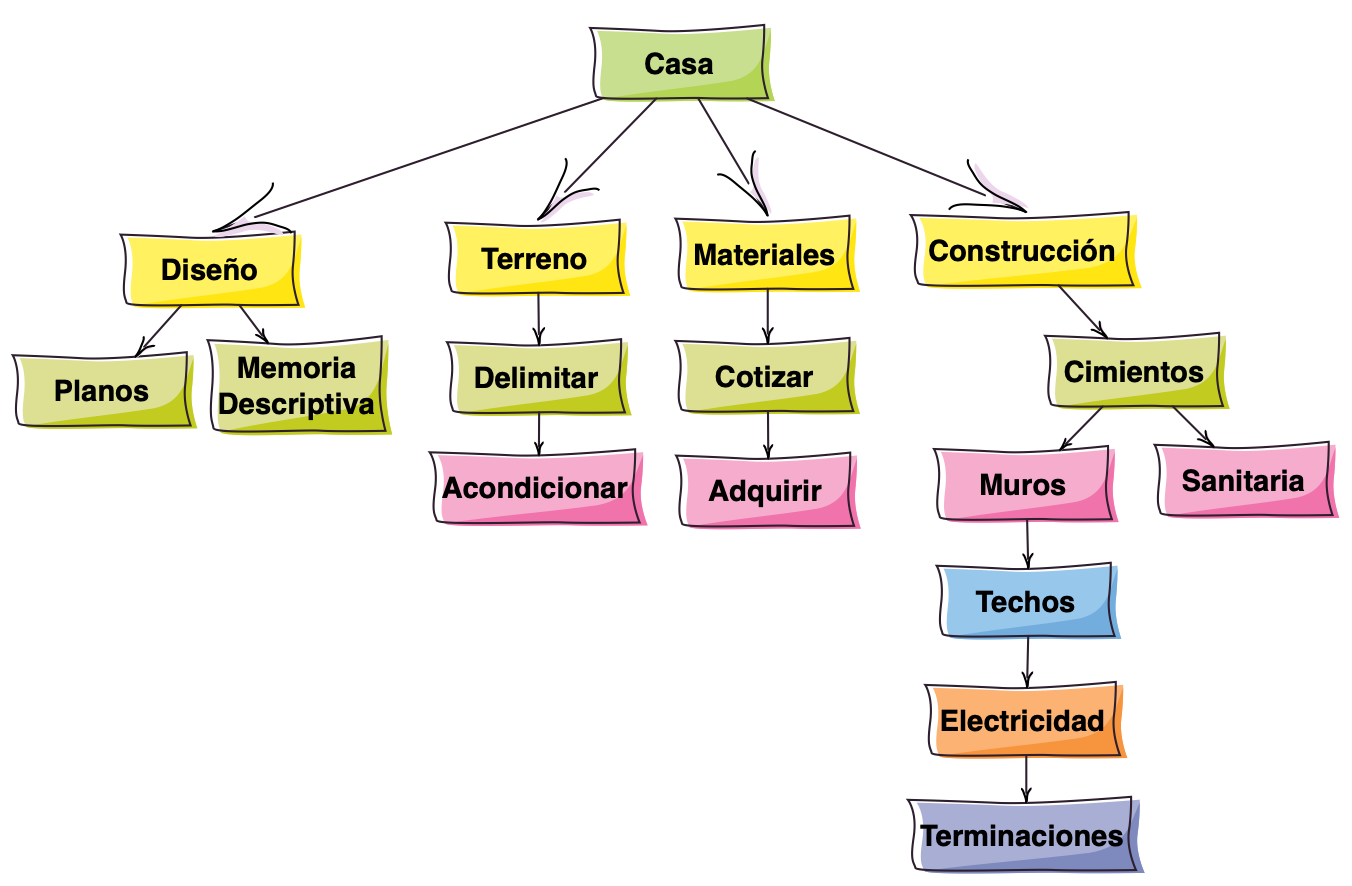
\includegraphics[height=7.5cm]{images/wbscasa}
\end{center}

\vspace{-3cm}
{\scriptsize
Nota:
\begin{enumerate}\justifying
  \item No se representan relaciones de precedencia.
  \item Es usual presentarlo (en lo posible) en orden de ejecución.
\end{enumerate}}

\end{frame}


\subsubsection{Gantt}
\begin{frame}[fragile]
\frametitle{\textbf{Carta Gantt}}
\justifying
 \begin{itemize}\justifying
  \item El programa Gantt consiste en la graficación secuencial con barras horizontales en un calendario cuya unidad de tiempo pueden ser horas, días, meses, u otra que se requiera.
  \item Estos gráficos son muy prácticos para la programación de un trabajo de no más de 50 actividades.
  \item En caso de mayor número debería desglosarse en actividades más generales de modo de no sobrepasar dichas cifras.
  \item Requiere de un estudio detallado para verificar que el inicio del proyecto y partes de ella estén perfectamente coordinadas.
  \item No indica las dependencias o interconexiones entre las actividades.
\end{itemize}

\end{frame}

\begin{frame}[fragile]
\frametitle{\textbf{Ejemplo Carta Gantt: Casa}}
\justifying%\vspace{-4mm}
 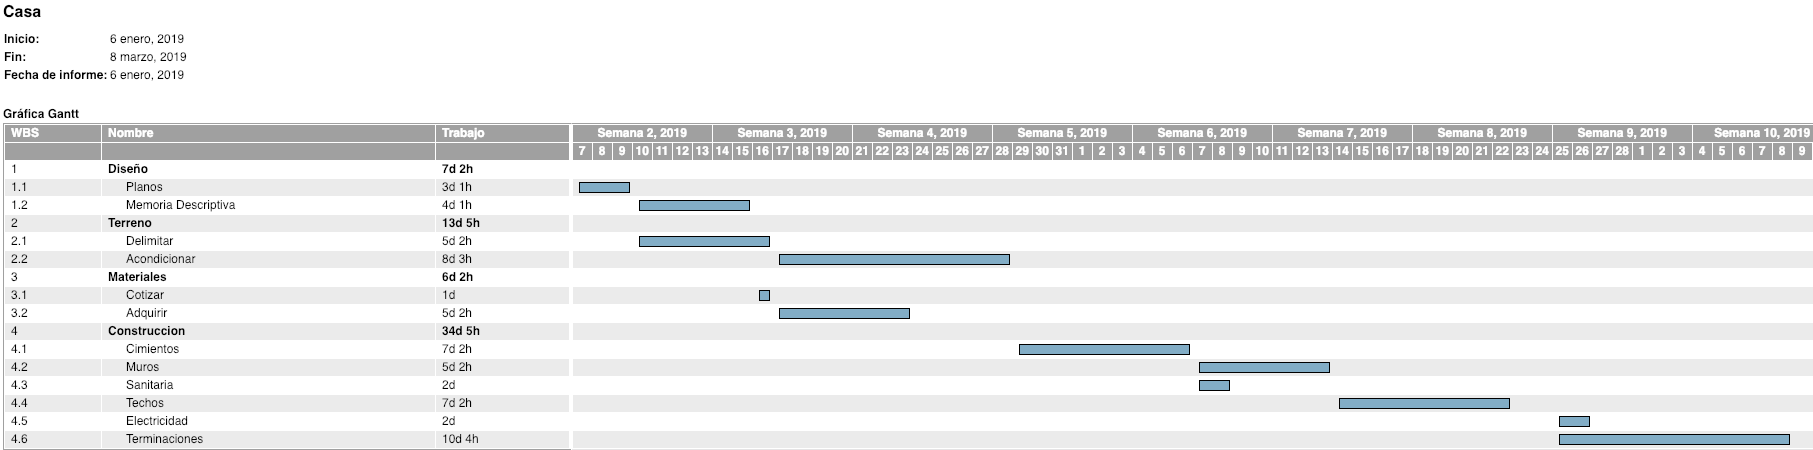
\includegraphics[width=15.5cm]{images/casagantt}
\end{frame}

\begin{frame}[fragile]
\frametitle{\textbf{Ejemplo Carta Gantt: Proyecto}}
\framesubtitle{Actividades y Tareas Codificadas}
\justifying%\vspace{-4mm}
 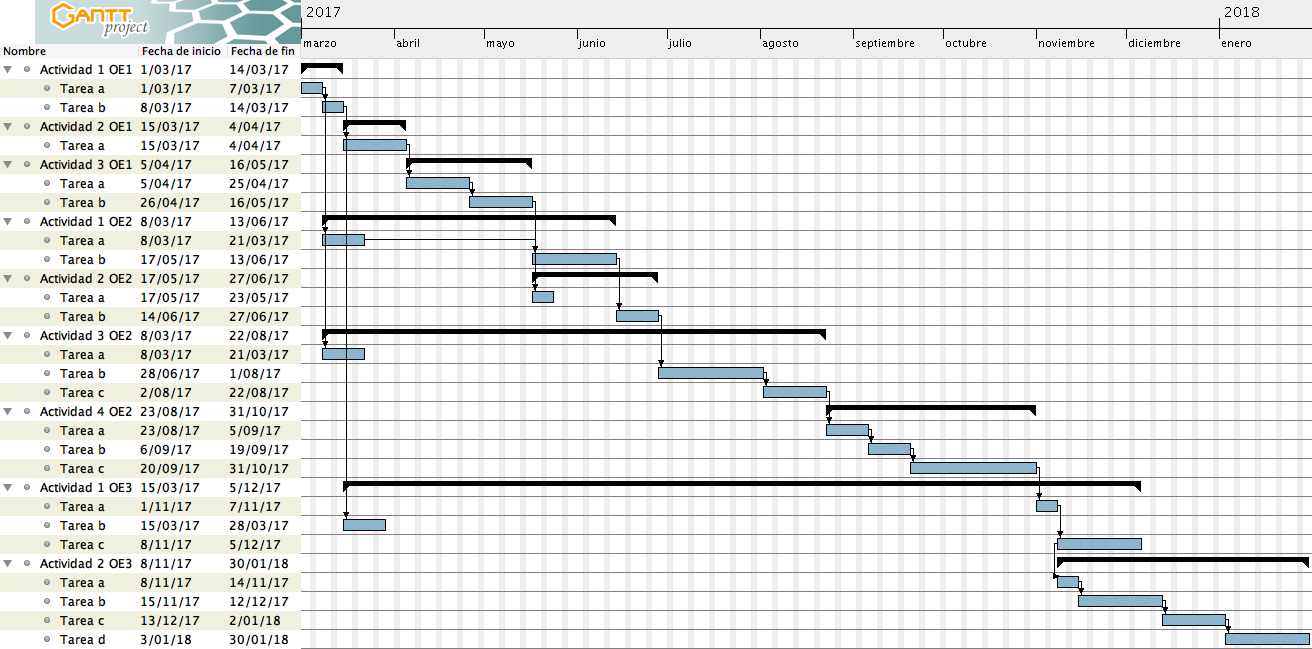
\includegraphics[width=14cm]{images/ganttresumen}
\end{frame}


\begin{frame}[fragile]
\frametitle{\textbf{Ejemplo Carta Gantt: Proyecto}}
\framesubtitle{Actividades Codificadas y Tareas sin Codificar}
\justifying
 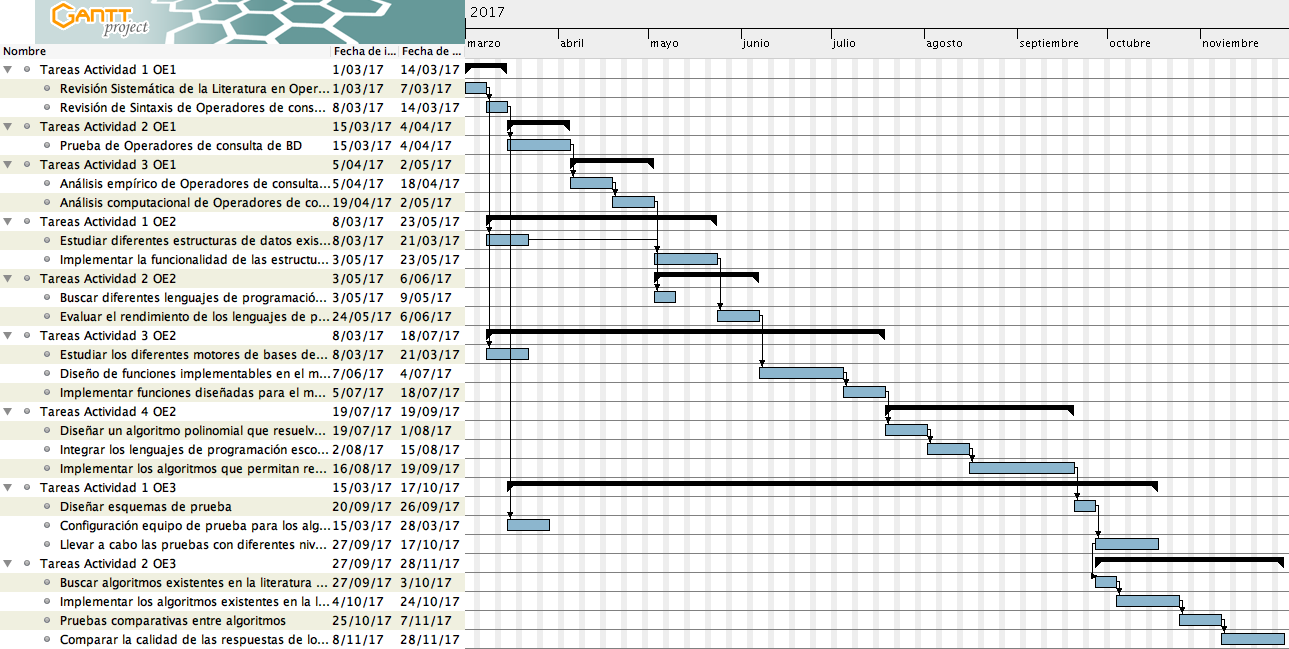
\includegraphics[width=14cm]{images/ProyectoGantt}
\end{frame}


\begin{frame}[fragile]
\frametitle{\textbf{Cuadro de Actividades (CPM)}}
\framesubtitle{Duración de Tareas y Dependencias}
\justifying
 \begin{itemize}\justifying
  \item Se consideran:
  \begin{itemize}\justifying
  \item Las hojas del WBS (Actividades) o la Carta Gantt
  \item Las relaciones de precedencia entre ellas.
  \item Una actividad no puede comenzar hasta que las precedentes hayan concluido.
\end{itemize}

  \item Modelo del proyecto: Actividades, Precedencias, Duraciones.
\end{itemize}


\end{frame}

\begin{frame}[fragile]
\frametitle{\textbf{Ejemplo Cuadro de Actividades: Casa}}
\justifying
\begin{center}
\begin{tabular}{|c|c|c|c|c|}\hline
  \textbf{Actividad}&\textbf{Duración} &\textbf{Después de} & \textbf{Simultanea a} & \textbf{Antes de}\\\hline
A (1.1) & 3& -&-&B\\\hline
B (1.2) & 4& A&-&D\\\hline
C (2.1) & 5& A&B&D\\\hline
D (2.2) & 8& E&F&G\\\hline
E (3.1) & 1& B&-&F\\\hline
F (3.2) & 5& E&D&G\\\hline
G (4.1) & 7& D&-&I\\\hline
H (4.2) & 5& G&I&J\\\hline
I  (4.3)& 2& G&H&-\\\hline
J  (4.4)& 7& H&-&K\\\hline
K (4.5) & 2& J&L&-\\\hline
L (4.6) & 10&J&K&-\\\hline
\end{tabular}
\end{center}
\end{frame}

\begin{frame}[fragile]
\frametitle{\textbf{Ejemplo Cuadro de Actividades: Proyecto}}
\justifying
\begin{center}
\begin{tabular}{|c|c|c|c|c|}\hline
  \textbf{Actividad}&\textbf{Duración} &\textbf{Después de} & \textbf{Simultanea a} & \textbf{Antes de}\\\hline
A1OE1A& 1S&-      &-&A1OE1B\\\hline
A1OE1B& 1S&A1OE1A &-&A2OE1A\\\hline
A2OE1A& 3S&A1OE1B &-&A3OE1A\\\hline
A3OE1A& 3S&A2OE1A &-&A3OE1B\\\hline
A3OE1B& 3S&A3OE1A &-&A1OE2B\\\hline
A1OE2A& 2S&A1OE1A &-&A1OE2B\\\hline
A1OE2B& 4S&A3OE1B &-&A2OE2B\\\hline
A2OE2A& 1S&A3OE1B &-&-\\\hline
A2OE2B& 2S&A1OE2B &-&A3OE2B\\\hline
A3OE2A& 2S&A1OE1A &-&-\\\hline
A3OE2B& 5S&A2OE2B &-&A3OE2C\\\hline
A3OE2C& 3S&A3OE2B &-&A4OE2A\\\hline
\end{tabular}
\end{center}
\end{frame}

\begin{frame}[fragile]
\frametitle{\textbf{Ejemplo Cuadro de Actividades: Proyecto}}
\justifying
\begin{center}
\begin{tabular}{|c|c|c|c|c|}\hline
  \textbf{Actividad}&\textbf{Duración} &\textbf{Después de} & \textbf{Simultanea a} & \textbf{Antes de}\\\hline
A4OE2A& 2S&A3OE2C &-&A4OE2B\\\hline
A4OE2B& 2S&A4OE2A &-&A4OE2C\\\hline
A4OE2C& 6S&A4OE2B &-&A1OE3A\\\hline
A1OE3A& 1S&A4OE2C &-&A1OE3C\\\hline
A1OE3B& 2S&A1OE1B &-&-\\\hline
A1OE3C& 4S&A1OE3A &-&-\\\hline
A2OE3A& 1S&A1OE3A &-&A2OE3B\\\hline
A2OE3B& 4S&A2OE3A &-&A2OE3B\\\hline
A2OE3C& 3S&A2OE3B &-&A2OE3C\\\hline
A2OE3D& 4S&A2OE3C &-&-\\\hline
\end{tabular}
\end{center}
\end{frame}

\section{Marco Teórico}
\begin{frame}[fragile]
\frametitle{\textbf{Marco Teórico}}
\justifying
\begin{itemize}

 \item Permite determinar si se justifica o no realizar el proyecto, ya que se pueden encontrar alternativas.
  \item Ayuda a prevenir errores que se han cometido en otros desarrollos, como también encontrar mejoras.
 \item Centra al desarrollador en el problema, para evitar desviaciones del planteamiento original.

\item Considera una \naranjo{revisión bibliográfica} que consiste en detectar, obtener y consultar la bibliografía, Sistemas y otros materiales que pueden ser útiles para los propósitos del desarrollo.
\end{itemize}

\end{frame}
%%%%%%%%%%%%%%%%%%%%%%%%%%%%%%
%%%%%%%%%%%%%%%%%FIN DOCUMENTO
\end{document}
